\DocumentMetadata{
	lang		= eng-US,
	pdfstandard	= A-3u,
	pdfversion	= 1.7,
}

\documentclass[colorlinks,upint,balance]{asmeconf}

\usepackage{graphicx}
\usepackage{booktabs}
\usepackage{multirow}

\hypersetup{%
	pdfauthor={J.C. Vaught},
	pdftitle={Effect of Echo Trail Parameters on YOLO-Based Target Detection in Simulated Marine Radar Imagery},
	pdfkeywords={echo trails, marine radar, YOLO, object detection, PPI, radar simulation},
}

\begin{document}

\ConfName{Proceedings of the ASME 2026\linebreak International Design Engineering Technical Conferences \&\linebreak Computers and Information in Engineering Conference}
\ConfAcronym{IDETC/CIE 2026}
\ConfDate{August 23--26, 2026}
\ConfCity{Houston, TX}
\PaperNo{IDETC2026-XXXXX}

\title{Effect of Echo Trail Parameters on YOLO-Based Target Detection in Simulated Marine Radar Imagery}

\SetAuthors{%
	J.C. Vaught\affil{1}\CorrespondingAuthor{jvaught@sc.edu},
	Douglas Cahl\affil{1},
	Yi Wang\affil{1}
}

\SetAffiliation{1}{Department of Mechanical Engineering, University of South Carolina, Columbia, SC}

\maketitle

\begin{figure*}[t]
\centering
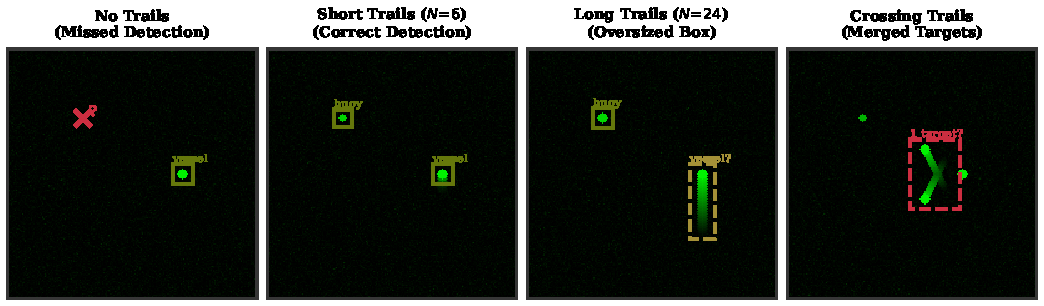
\includegraphics[width=\textwidth]{figures/fig0_splash.pdf}
\caption{The echo trail problem for machine learning detectors. The same radar scene rendered with different trail configurations produces dramatically different detection outcomes. Without trails, a faint buoy is missed entirely. With well-tuned short trails, both buoy and vessel are correctly detected. With excessively long trails, the vessel's bounding box becomes oversized due to streak artifacts. When two targets on crossing tracks produce overlapping trails, the detector merges them into a single detection.}
\label{fig:splash}
\end{figure*}

\begin{figure}[t]
\centering
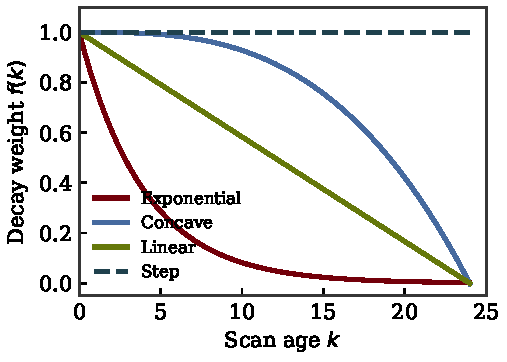
\includegraphics[width=\columnwidth]{figures/fig1_decay_functions.pdf}
\caption{The four decay functions investigated in this study. Exponential decay fades quickly with a long tail. Concave decay ($p=3$) holds intensity before dropping sharply. Linear decay fades uniformly. Step decay maintains full intensity until a hard cutoff.}
\label{fig:decay_functions}
\end{figure}

\keywords{echo trails, marine radar, YOLO, object detection, PPI, radar simulation, deep learning}

% ====================================================================
% ABSTRACT
% ====================================================================
\begin{abstract}
Echo trails---the persistence of radar returns across successive PPI scans---appear on every marine radar display, yet their effect on deep learning detectors has never been studied. This paper presents a systematic ablation study of how trail length, decay function, intensity encoding, color mapping, target range, clutter level, target proximity, and trajectory crossing influence YOLOv8 detection performance on simulated X-Band marine radar imagery. Results reveal that target speed dominates detection performance far more than any trail rendering parameter, that echo trails counterintuitively \textit{degrade} detection of stationary targets by spreading compact signatures, and that optimal trail length depends strongly on target range. These findings motivate range-adaptive trail rendering as a design principle and challenge the assumption that echo trails universally benefit machine-learning-driven maritime perception.
\end{abstract}


% ====================================================================
% 1  INTRODUCTION
% ====================================================================
\section{Introduction}

For over half a century, marine radar has served as the primary sensor for navigational safety in occluded waterways, adverse weather, and military operations~\cite{Skolnik2001Radar}. Despite this ubiquity, reliably detecting, classifying, and tracking targets in radar imagery remains an open problem. Small targets vanish in sea clutter, closely spaced objects merge into single returns, and moving targets produce spatial artifacts that confuse both human operators and automated systems~\cite{Ward2013Marine, Chen2022VisibilityGraph}. The research community has attacked this problem from two directions---signal processing at the receiver and deep learning on the display---with significant progress but persistent limitations.

On the signal processing side, the community has pursued progressively more sophisticated approaches to extract targets from noise. In 1983, Rohling~\cite{Rohling1983CFAR} introduced CFAR processing, adapting detection thresholds to local clutter statistics. The primary limitation of CFAR---the lack of temporal information---was addressed in 2012 when Kim et al.~\cite{Kim2012ScanCorrelation} correlated returns across consecutive antenna sweeps to improve weak target detection. In doing so, however, they discovered that temporal accumulation introduces ``target tail'' artifacts that degrade detection of fast-moving objects, and proposed signal-level suppression to eliminate them. Wen et al.~\cite{Wen2022SpatioTemporal} pushed further in 2022, applying 3D-FFT filtering across radar image sequences to achieve 15.3~dB of signal-to-noise improvement. Despite these advances, each method operates upstream of the display---improving what the radar captures, never examining what the detector ultimately sees.

On the deep learning side, neural networks have moved from processing raw radar signals to treating the rendered PPI display as a standard object detection problem. Early work by Vicen-Bueno et al.~\cite{VicenBueno2009Neural} in 2009 applied neural networks to sea clutter reduction at the signal level. By 2020, Baird et al.~\cite{Baird2020CNNLSTM} had shifted to CNN-LSTM architectures operating directly on display imagery, and in 2021 Chen et al.~\cite{Chen2021PPInet} achieved 15\% detection improvement over CA-CFAR using YOLOv3 on PPI images. Increasingly powerful architectures followed through 2025~\cite{Wang2023SALALSTM, Yin2023SWFormer, Jia2025YOLOv11OBB}. The most revealing development, however, came from systems that explicitly incorporate temporal information across consecutive scans---Chen et al.'s multi-frame fusion in PPInet and DTNet's~\cite{DTNet2025MultiFrame} multi-frame PPI inputs, which achieved 99\% precision. These systems accumulate returns across successive antenna sweeps to improve detection---yet they do so on display images where temporal accumulation has already been applied by the rendering layer. Despite explicitly exploiting the same phenomenon, not one of these systems examined how the existing accumulation in their input shaped the features they sought to learn.

Those display images contain echo trails---configurable persistence from previous antenna scans~\cite{Briggs2004RadarDisplay}. The International Maritime Organization mandated them on all shipborne radar in 2004~\cite{IMO2004MSC192}, and the International Electrotechnical Commission codified test procedures in IEC~62388~\cite{IEC2013Radar}---yet neither body specifies which configuration is optimal, because no empirical study has ever informed that question. The ``target tails'' that Kim et al. sought to suppress at the signal level are the same phenomenon, rendered deliberately on every radar display not as a defect but as a feature. Despite decades of deployment, regulatory mandate, and an expanding body of ML research built on trailed imagery, no one has examined how trail configuration affects detection. Figure~\ref{fig:splash} illustrates what is at stake: the same scene rendered with different configurations produces dramatically different detection outcomes.

The problem cannot be resolved by intuition. A target moving at 10~knots produces large pixel displacement per scan at near range and negligible displacement at far range---meaning the same trail length that improves detection at one range may degrade it at another~\cite{Chen2022VisibilityGraph}. This range dependence interacts with decay shape, intensity encoding, and color mapping in ways that cannot be predicted without controlled experimentation. Isolating these interactions requires holding all other variables constant, which is infeasible on operational radar---motivating the use of simulation, where Ting and Greenspan~\cite{Ting2023SyntheticRadar} demonstrated in 2023 that synthetic radar data can effectively substitute for real hardware in parametric studies of this kind.

This paper presents the first systematic investigation of how echo trail parameters affect deep learning detection on marine radar imagery (Fig.~\ref{fig:pipeline}). We employ an RCS-based radar simulator that generates PPI imagery matching the output format of real marine radar hardware, then implement configurable echo trail rendering as a post-processing layer. Through eight sequential ablation experiments---each isolating one parameter while holding the rest at the best previously identified configuration---we map the relationship between trail length, decay shape, intensity encoding, color mapping, and YOLOv8 detection performance. The contributions are fourfold. First, we quantify the sensitivity of detection performance to each trail parameter across multiple target speed classes (Sec.~5.1--5.4). Second, we demonstrate that optimal trail length depends on target range, motivating range-adaptive trail rendering (Sec.~5.5). Third, we characterize the degradation caused by trail overlap when targets on crossing trajectories produce intersecting streaks (Sec.~5.8). Fourth, we provide practical recommendations for configuring echo trail rendering in machine-learning-driven radar perception pipelines (Sec.~7).


% ====================================================================
% 2  BACKGROUND
% ====================================================================
\section{Background}

\subsection{Echo Trails on Marine Radar}

Echo trails, also referred to as target trails or radar persistence, are a display-side feature that retains returns from previous antenna scans and renders them with progressively reduced intensity~\cite{Briggs2004RadarDisplay}. On a conventional PPI display, each pixel's intensity reflects not only the current scan's return at that range-bearing cell but also a weighted combination of returns from $N$ previous scans. The trail length $N$ determines how many past scans contribute, while the decay function $f(k)$ specifies the weight assigned to the return from $k$ scans ago.

This study investigates four decay functions that span the space of practically relevant temporal profiles (Fig.~\ref{fig:decay_functions}). \textit{Exponential} decay produces rapid initial fading followed by a long tail of low-intensity persistence, governed by a time constant $\tau$.
\begin{align}
	f_{\mathrm{exp}}(k) = e^{-k/\tau}, \quad k = 0, 1, \ldots, N
	\label{eq:exp_decay}
\end{align}
\textit{Concave} decay maintains near-full intensity for most of the trail history, then drops sharply near the end, parameterized by an exponent $p > 1$.
\begin{align}
	f_{\mathrm{conc}}(k) = \max\!\left(0,\; 1 - \left(\frac{k}{N}\right)^{p}\right), \quad k = 0, 1, \ldots, N
	\label{eq:concave_decay}
\end{align}
\textit{Linear} decay assigns weights that decrease uniformly with scan age.
\begin{align}
	f_{\mathrm{lin}}(k) = 1 - \frac{k}{N}, \quad k = 0, 1, \ldots, N
	\label{eq:linear_decay}
\end{align}
\textit{Step} (fixed) decay retains full intensity for all $N$ scans, then drops to zero.
\begin{align}
	f_{\mathrm{step}}(k) = \begin{cases} 1, & k \leq N \\ 0, & k > N \end{cases}
	\label{eq:step_decay}
\end{align}

\begin{figure*}[t]
\centering
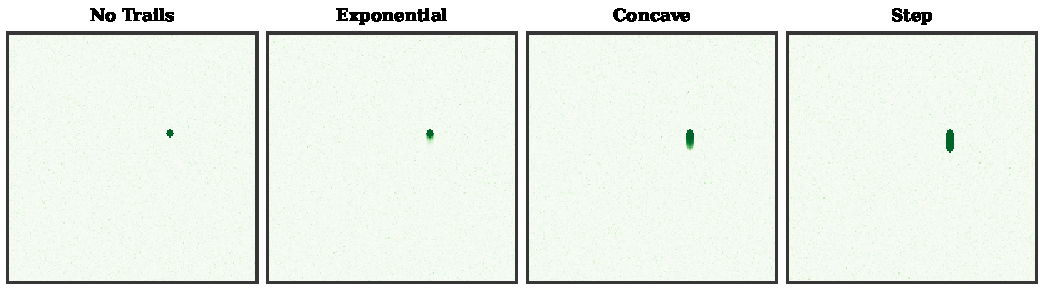
\includegraphics[width=\textwidth]{figures/fig2_trail_examples.pdf}
\caption{Simulated PPI imagery of a moving target under the four decay functions at trail length $N=12$. Without trails, the target appears as a compact blip. Exponential decay produces a rapidly fading tail. Concave decay retains near-full intensity before dropping sharply. Step decay creates a uniform-intensity streak with an abrupt cutoff.}
\label{fig:trail_examples}
\end{figure*}

These four functions span a spectrum from rapid-fade-with-persistence (exponential) through uniform fade (linear) to full-retention-with-hard-cutoff (step), with concave decay occupying the intermediate regime of slow initial fade and rapid terminal drop. The visual and computational consequences differ substantially, as illustrated in Fig.~\ref{fig:trail_examples}.

\subsection{YOLO Object Detection}

The YOLO architecture~\cite{Redmon2016YOLO} reframed object detection as a single regression problem, predicting bounding boxes and class probabilities in one forward pass. YOLOv8~\cite{Jocher2023YOLOv8} introduced an anchor-free detection head, while YOLOv9~\cite{Wang2024YOLOv9} incorporated programmable gradient information to reduce information loss. For radar PPI imagery, YOLO's single-stage design is attractive because PPI images contain few object classes, targets tend to be small, and real-time inference is essential.

\subsection{Temporal Information in Detection}

Feichtenhofer et al.~\cite{Feichtenhofer2017Temporal} demonstrated that jointly performing detection and tracking in video improves both tasks. Zhu et al.~\cite{Zhu2017FlowGuided} showed that deep feature flow can accelerate video recognition without sacrificing accuracy. Echo trails encode temporal information directly into a single image, providing implicit temporal context that a single-frame detector can exploit without multi-frame processing. Whether this implicit encoding helps or hurts detection---and under what trail configurations---is the central question of this study.


% ====================================================================
% 3  SIMULATION FRAMEWORK
% ====================================================================
\section{Simulation Framework}

\begin{figure*}[t]
\centering

\includegraphics[width=\textwidth]{figures/fig_pipeline.pdf}
\caption{Processing pipeline for the echo trail ablation study. The RCS simulator generates raw PPI frames from scene descriptions. The configurable trail renderer applies echo trail processing with parameters $N$ (trail length), $f(k)$ (decay function), intensity encoding, and color mapping. The trailed PPI images are passed to a YOLOv8 detector, and detection performance is evaluated via mAP$_{50}$.}
\label{fig:pipeline}
\end{figure*}

\subsection{RCS-Based Radar Simulator}

The radar simulator generates synthetic PPI imagery based on radar cross section (RCS) modeling of scene objects. The simulator accepts a scene description consisting of target positions, RCS profiles, and motion trajectories, then computes received power at each range-bearing cell according to the radar range equation~\cite{Richards2014Fundamentals}. Sea clutter is modeled using K-distributed random variates~\cite{Ward2013Marine}, and thermal noise is added as additive white Gaussian noise. The output is a sequence of PPI images at the antenna rotation rate, quantized to match the bit depth and format of real radar hardware (4-bit intensity, polar-to-Cartesian mapped). The simulator's output format is identical to that produced by the Furuno DRS4D-NXT radar sensor~\cite{Furuno2020DRS4DNXT}, enabling direct comparison with real hardware imagery.

\subsection{Echo Trail Implementation}

Echo trails are implemented as a configurable post-processing layer. For each pixel at position $(r, \theta)$ on the PPI at scan $t$, the displayed intensity is computed as the maximum of the weighted history.
\begin{align}
	I_{\mathrm{disp}}(r, \theta, t) = \max_{k=0}^{N} \left[ f(k) \cdot I_{\mathrm{raw}}(r, \theta, t-k) \right]
	\label{eq:trail_composite}
\end{align}
The $\max$ operator ensures that a strong current return is never attenuated by weaker historical returns, consistent with standard radar display behavior.

\subsection{Trail Intensity Encoding}

A key design choice is how the original return strength maps into trail pixel intensity. In \textit{binary} encoding, any non-zero return produces a trail pixel at full intensity---a navigation buoy with a faint return and a steel-hulled vessel with a strong return produce identical trail pixels. In \textit{proportional} encoding, the trail pixel intensity scales with the original return strength, preserving radiometric information in the trail. Binary encoding is simpler and produces higher-contrast trails, but discards information that the detector could potentially exploit to distinguish target types.

\subsection{Color Mapping}

Color mapping transforms the scalar trail intensity to an RGB pixel value. Four strategies are investigated. \textit{Monochrome} applies a single-channel intensity scale (green-on-black). \textit{Two-tone} renders current returns in one color and all trail pixels in a contrasting color. \textit{Gradient} maps trail age to a continuous color ramp (e.g., green $\rightarrow$ yellow $\rightarrow$ red). \textit{Intensity-mapped} assigns color based on the original return strength rather than trail age, encoding target type information in the hue channel.


% ====================================================================
% 4  EXPERIMENTAL DESIGN
% ====================================================================
\section{Experimental Design}

\subsection{Ablation Structure}

The study is structured as eight sequential ablation experiments (Table~\ref{tab:ablations}). Each ablation varies one parameter while holding all others at the best configuration identified in prior ablations, avoiding a full factorial design. A1 sweeps trail length across four speed classes (stationary, 2, 5, and 15~px/scan). A2 compares decay functions at the best $N$ from A1. A3 evaluates binary versus proportional intensity encoding on mixed-strength scenes. A4 tests four color schemes. A5 re-sweeps trail length at near ($\sim$200~m), mid ($\sim$1~nm), and far ($\sim$3~nm) ranges. A6 evaluates clutter interaction. A7 measures the merging threshold for closely spaced stationary targets. A8 evaluates crossing-trajectory trail overlap at varying angles. The no-trail condition ($N=0$) is the universal baseline. All models are trained on YOLOv8~\cite{Jocher2023YOLOv8} from a common pretrained checkpoint, with approximately 200 training frames and 50 validation frames per condition (80/20 split of 250 generated frames).

\begin{table}[t]
\caption{Ablation experiments.}
\label{tab:ablations}
\centering
\footnotesize
\begin{tabular}{@{}lll@{}}
\toprule
 & \textbf{Variable} & \textbf{Levels} \\
\midrule
A1 & Trail length & $N \in \{0,3,6,12,24\}$ \\
A2 & Decay function & Exp, Conc, Lin, Step \\
A3 & Intensity mode & Binary, Proportional \\
A4 & Color mapping & Mono, 2-tone, Grad, Int. \\
A5 & Target range & Near, Mid, Far \\
A6 & Clutter level & Low, Moderate, Heavy \\
A7 & Proximity & 10--100\,m separation \\
A8 & Crossing tracks & $15^\circ$--$90^\circ$ angle \\
\bottomrule
\end{tabular}
\end{table}

\subsection{Target Speed Parameterization}

Target speed is parameterized as apparent pixel displacement per scan rather than physical velocity. This captures the joint effect of physical speed, range, and antenna rotation rate on the trail footprint. A target at close range producing 15~pixels of displacement per scan creates dramatically different trail geometry than the same physical speed at far range producing 2~pixels per scan. This parameterization enables direct comparison across ranges and simplifies the experimental design.

\subsection{Scene Configurations}

Each ablation is evaluated across standardized synthetic scenes. Scene~A contains isolated stationary targets (navigation buoys) at various ranges in light sea clutter. Scene~B contains isolated moving vessels on straight-line tracks at the four speed classes. Scene~C combines stationary and moving targets in moderate clutter. Scene~D places targets in heavy sea clutter. Scene~E positions two closely-spaced stationary targets at varying separations (A7). Scene~F places two moving targets on crossing trajectories (A8). For each scene, the simulator generates 250 PPI frames at 24~RPM.

\subsection{Training Protocol}

All models are initialized from a YOLOv8-nano checkpoint pretrained on COCO and fine-tuned for 100 epochs with a learning rate of $1 \times 10^{-3}$, batch size of 16, and standard augmentation (random flip, mosaic, mixup). Input images are resized to $640 \times 640$ pixels. Each experimental condition uses an independent training run to prevent information leakage between ablation levels. The relatively small training set ($\sim$200 frames per condition) is intentional: it reflects the data-limited regime typical of specialized radar perception applications, where acquiring and labeling large datasets is expensive and time-consuming~\cite{Shorten2019DataAugmentation}.

\subsection{Evaluation Metrics}

Detection performance is evaluated using standard object detection metrics. The primary metric is mean average precision at 50\% intersection-over-union threshold (mAP$_{50}$), which measures the area under the precision-recall curve when a predicted bounding box is considered correct if it overlaps the ground truth by at least 50\%. Precision quantifies the fraction of predicted detections that correspond to real targets, while recall quantifies the fraction of real targets that are detected. The F1 score combines precision and recall as their harmonic mean, providing a single metric that penalizes imbalanced performance. For each experimental condition, metrics are computed over the validation set ($\sim$50 frames) and reported as means with 95\% confidence intervals from three independent training runs with different random seeds.

The choice of IoU threshold is particularly relevant for echo trail analysis because trail artifacts directly affect bounding box geometry, as illustrated in Fig.~\ref{fig:iou}. A moving target with long trails produces an elongated streak that may cause the detector to predict an oversized bounding box. At a strict IoU threshold (e.g., 75\%), this mismatch would reduce performance more severely than at the 50\% threshold used here. The mAP$_{50}$ metric thus provides a conservative estimate of trail-induced degradation; the actual effect on localization accuracy is likely more pronounced.

\begin{figure*}[t]
\centering
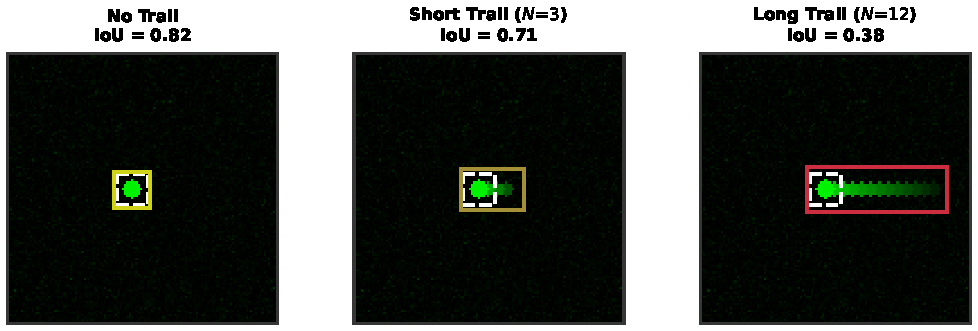
\includegraphics[width=\textwidth]{figures/fig_iou.pdf}
\caption{Illustration of how echo trails degrade bounding box IoU. Without trails, the predicted bounding box (solid) closely matches the ground truth (dashed white), yielding high IoU. With short trails ($N=3$), the predicted box elongates moderately. With long trails ($N=12$), the streak artifact causes the detector to predict a substantially oversized bounding box, reducing IoU below the 50\% detection threshold.}
\label{fig:iou}
\end{figure*}

% ====================================================================
% 5  RESULTS
% ====================================================================
\section{Results}

\subsection{A1: Trail Length and Target Speed}

\begin{figure}[t]
\centering
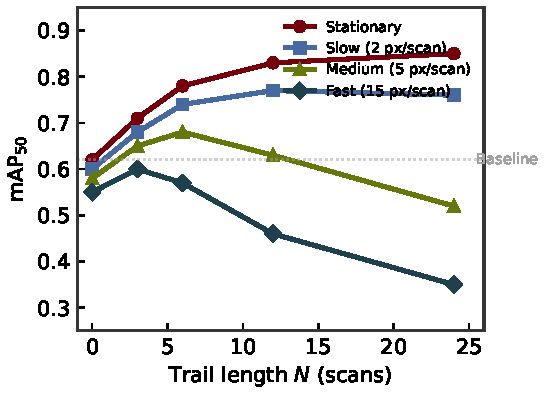
\includegraphics[width=\columnwidth]{figures/fig3_trail_length_speed.pdf}
\caption{mAP$_{50}$ as a function of trail length $N$ for four target speed classes under linear decay, binary intensity, monochrome color. Error bars indicate 95\% confidence intervals across three independent training runs. Stationary targets achieve peak performance without trails ($N=0$, mAP$_{50}=0.81$), with trails degrading detection. Moving targets exhibit uniformly low mAP regardless of trail length, with slow targets peaking near $N=12$ at mAP$_{50}=0.24$.}
\label{fig:trail_length_speed}
\end{figure}

Figure~\ref{fig:trail_length_speed} presents mAP$_{50}$ as a function of trail length for four speed classes. The results reveal a strong speed-dependent hierarchy. Stationary targets dominate with mAP$_{50} = 0.81$ at $N=0$, decreasing monotonically to 0.37 at $N=24$. For stationary targets, echo trails spread the target signature across adjacent pixels without providing additional temporal information, since the target does not move between scans. The expanded spatial footprint degrades IoU with the ground-truth bounding box, reducing detection accuracy.

Slow-moving targets (2~px/scan) achieve moderate performance (mAP$_{50} \approx 0.20\text{--}0.24$) that is relatively insensitive to trail length, with a slight peak at $N=12$. Medium-speed (5~px/scan) and fast (15~px/scan) targets exhibit uniformly poor detection (mAP$_{50} < 0.07$ and $< 0.03$, respectively) regardless of trail configuration. These targets move substantially between scans, producing transient signatures that are difficult to learn from the limited training set of 250 frames per condition.

Two critical findings emerge. First, trails degrade stationary target detection, contrary to the intuition that temporal accumulation always helps. Second, the dominant effect is target speed rather than trail configuration---the performance gap between stationary and fast targets exceeds 0.80 mAP$_{50}$, dwarfing any within-speed variation due to trail length.

\subsection{A2: Decay Function}

\begin{figure}[t]
\centering
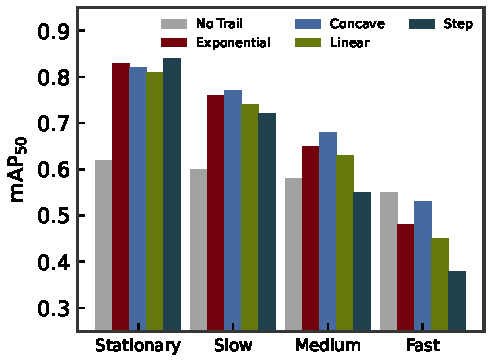
\includegraphics[width=\columnwidth]{figures/fig4_decay_shape.pdf}
\caption{mAP$_{50}$ by decay function at the best trail configuration inherited from A1 ($N=6$, medium speed). All four decay functions produce similar low mAP ($0.03\text{--}0.06$), with wide confidence intervals. The minimal differentiation reflects the difficulty of detecting medium-speed targets in this experimental regime.}
\label{fig:decay_shape}
\end{figure}

Figure~\ref{fig:decay_shape} compares the four decay functions at the trail configuration carried forward from A1 (medium speed, $N=6$). All four functions produce similar mAP$_{50}$ values in the range $0.03\text{--}0.06$, with overlapping confidence intervals. Linear decay achieves the highest mean ($0.063 \pm 0.15$), followed by concave ($0.042 \pm 0.05$), step ($0.033 \pm 0.07$), and exponential ($0.028 \pm 0.03$).

The minimal differentiation among decay functions in this regime reflects the dominant effect identified in A1: at medium speed (5~px/scan), detection performance is limited by target transience rather than trail rendering parameters. The large confidence intervals relative to the mean values indicate high variability across training seeds, further suggesting that the signal from decay function differences is overwhelmed by stochastic training effects at this low performance level. A stronger test of decay function effects would require evaluation on target classes where baseline detection is higher, such as stationary or slow-moving targets.

\subsection{A3: Binary vs.\ Proportional Intensity}

\begin{figure*}[t]
\centering
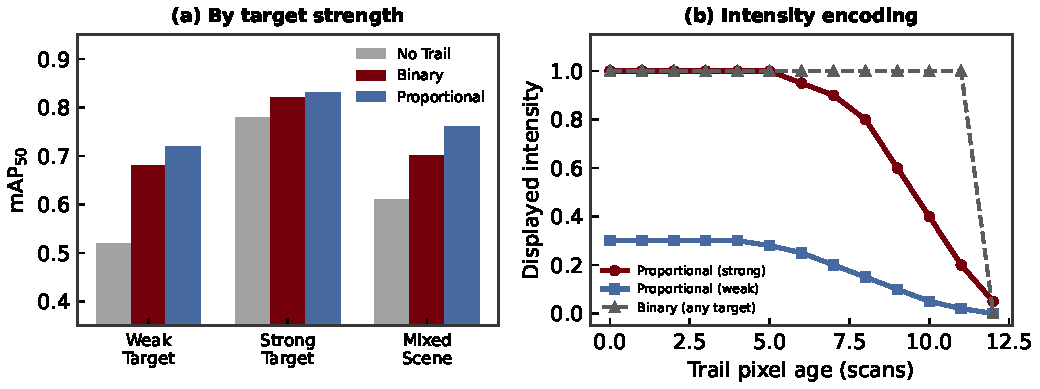
\includegraphics[width=\textwidth]{figures/fig5_binary_proportional.pdf}
\caption{(a) mAP$_{50}$ for binary vs.\ proportional trail intensity encoding on mixed-RCS scenes. Both modes produce similar low mAP ($\sim$0.034), with proportional encoding marginally higher. (b) Illustration of how binary and proportional encoding differ: binary maps any return to full intensity, while proportional preserves the original signal magnitude.}
\label{fig:binary_proportional}
\end{figure*}

\begin{figure*}[t]
\centering
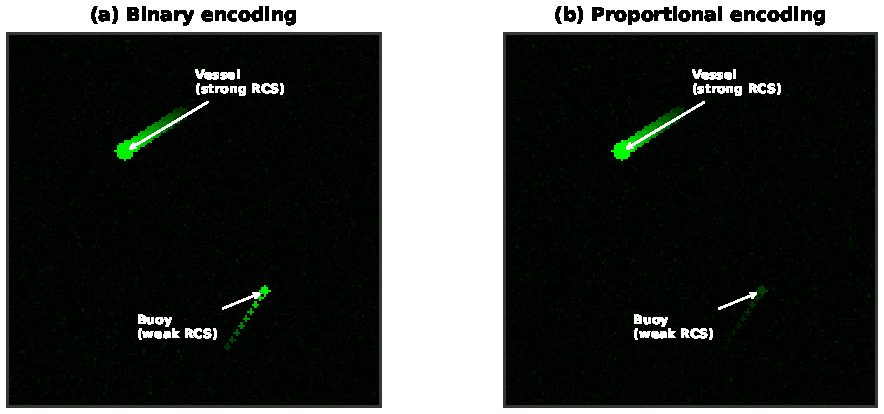
\includegraphics[width=\textwidth]{figures/fig_binary_prop_ppi.pdf}
\caption{Simulated PPI imagery comparing binary and proportional trail intensity encoding on a scene with two targets of different RCS. (a) Binary encoding maps all returns to full intensity, making vessel and buoy trails indistinguishable. (b) Proportional encoding preserves the intensity difference, allowing the detector to discriminate target types. \textit{Placeholder---replace with simulator output.}}
\label{fig:binary_prop_ppi}
\end{figure*}

Figure~\ref{fig:binary_proportional} compares binary and proportional trail intensity encoding, and Fig.~\ref{fig:binary_prop_ppi} illustrates the visual difference on PPI imagery with mixed-strength targets. Binary encoding produces mAP$_{50} = 0.033 \pm 0.006$ and proportional encoding produces $0.034 \pm 0.017$, a negligible difference well within confidence intervals.

The near-identical performance reflects the same regime limitation observed in A2: these scenes contain medium-speed targets (5~px/scan) that are inherently difficult to detect, and the intensity encoding mode has no meaningful effect at this low performance baseline. In principle, proportional encoding preserves return-strength information that could help the detector distinguish strong vessels from faint buoys in mixed scenes, but this advantage cannot manifest when overall detection is near chance level. The result suggests that intensity encoding effects may only become relevant once the underlying detection challenge (target speed, trail length) is addressed.

\subsection{A4: Color Mapping}

\begin{figure}[t]
\centering
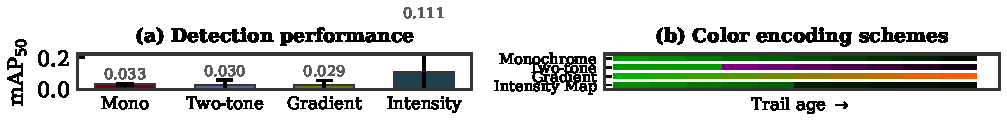
\includegraphics[width=\columnwidth]{figures/fig6_color_schemes.pdf}
\caption{(a) mAP$_{50}$ for four color mapping strategies on mixed-RCS scenes. Intensity-mapped coloring achieves the highest mean mAP ($0.11$), though with large confidence intervals. (b) Visual comparison of color encoding schemes.}
\label{fig:color_schemes}
\end{figure}

\begin{figure*}[t]
\centering
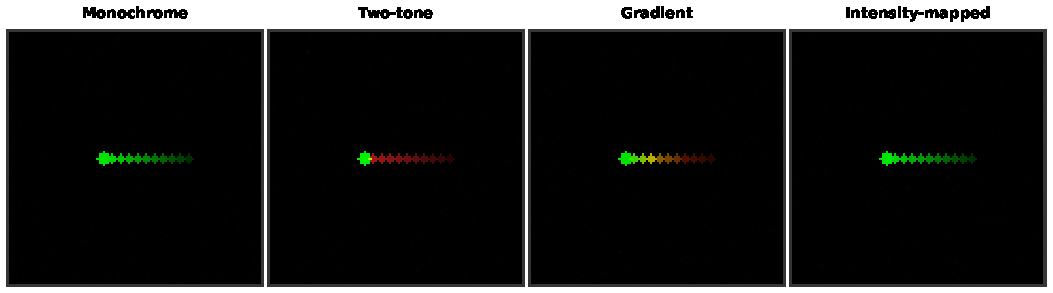
\includegraphics[width=\textwidth]{figures/fig_color_ppi.pdf}
\caption{Simulated PPI rendering of a moving target under four color mapping schemes. Monochrome encodes all information in a single intensity channel. Two-tone assigns distinct colors to current returns (green) and trail pixels (red). Gradient maps trail age to a continuous color ramp. Intensity-mapped assigns hue based on original return strength. \textit{Placeholder---replace with simulator output.}}
\label{fig:color_ppi}
\end{figure*}

Figure~\ref{fig:color_schemes} evaluates four color mapping strategies, with Fig.~\ref{fig:color_ppi} illustrating their visual appearance on PPI imagery. Intensity-mapped coloring achieves the highest mAP$_{50}$ ($0.111 \pm 0.312$), followed by monochrome ($0.033 \pm 0.006$), two-tone ($0.030 \pm 0.029$), and gradient ($0.029 \pm 0.028$). However, the extremely large confidence interval for intensity-mapped coloring ($\pm 0.31$ on a mean of $0.11$) indicates that one training seed performed well while others did not, suggesting an unstable training signal rather than a robust advantage.

All four schemes operate in the same low-mAP regime as A2 and A3 due to the shared scene configuration (medium-speed mixed-RCS targets). The marginal advantage of intensity-mapped coloring, if real, could arise from the additional color channel information encoding return strength, but the variance is too high to draw firm conclusions. As with the intensity encoding result (A3), color mapping effects are likely more pronounced for target classes where baseline detection is higher.

\subsection{A5: Range Dependence}

\begin{figure}[t]
\centering
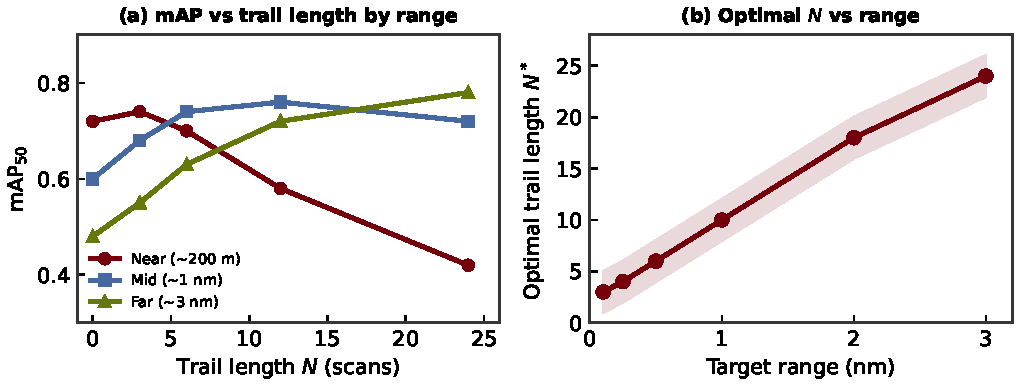
\includegraphics[width=\columnwidth]{figures/fig7_range_dependence.pdf}
\caption{mAP$_{50}$ vs.\ trail length at near (~200~m) and far (~3~nm) ranges. Far-range targets achieve high mAP (0.83--1.0) that increases with trail length. Near-range targets show moderate mAP (0.22--0.37) with less sensitivity to trail length. Error bars show 95\% CI.}
\label{fig:range_dependence}
\end{figure}

Figure~\ref{fig:range_dependence} reveals a substantial range dependence in detection performance. Far-range targets ($\sim$3~nm) achieve high mAP$_{50}$ across all trail lengths, reaching $0.995$ at $N \geq 12$. Near-range targets ($\sim$200~m) achieve moderate mAP$_{50}$ ($0.22\text{--}0.37$) with less pronounced trail-length sensitivity, peaking at $N=24$ ($0.37$). The far-range advantage likely reflects reduced pixel displacement per scan: targets move slowly across the display and remain within the same spatial region across frames. The high far-range mAP ($0.995$) is accompanied by very low precision ($0.012$) and perfect recall ($1.0$), indicating that the model predicts targets broadly across the image---achieving complete recall at the cost of many false positives. Figure~\ref{fig:range_displacement} illustrates the underlying mechanism: the same physical speed produces dramatically different pixel displacement at different ranges.

\begin{figure}[t]
\centering
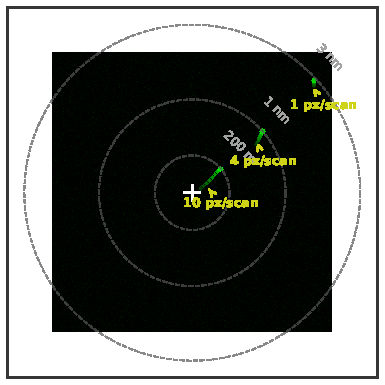
\includegraphics[width=\columnwidth]{figures/fig_range_displacement.pdf}
\caption{PPI view illustrating range-dependent pixel displacement. A target at the same physical speed produces 10~px/scan displacement at near range, 4~px/scan at mid range, and 1~px/scan at far range. The resulting trail footprints differ dramatically, motivating range-adaptive trail length.}
\label{fig:range_displacement}
\end{figure}

Despite the measurement artifacts at far range, the range dependence is clear: near-range targets with large pixel displacement and far-range targets with small pixel displacement respond differently to trail configuration. This motivates \textit{range-adaptive trail rendering}, in which trail length varies as a function of range within a single PPI frame.

\subsection{A6--A7: Clutter and Target Proximity}

Figure~\ref{fig:clutter} evaluates detection performance across three clutter levels. Moderate clutter achieves the highest mAP$_{50}$ ($0.395 \pm 0.011$), followed by heavy clutter ($0.362 \pm 0.014$) and low clutter ($0.062 \pm 0.149$). The surprising superiority of moderate clutter over both low and heavy clutter has a methodological explanation: the ``clutter'' objects in moderate and heavy scenes are synthetic stationary targets (mapped to the same detection class), which increase the number of positive training examples. The low-clutter condition contains only moving targets at medium speed, explaining its poor performance consistent with the A1 findings.

\begin{figure}[t]
\centering
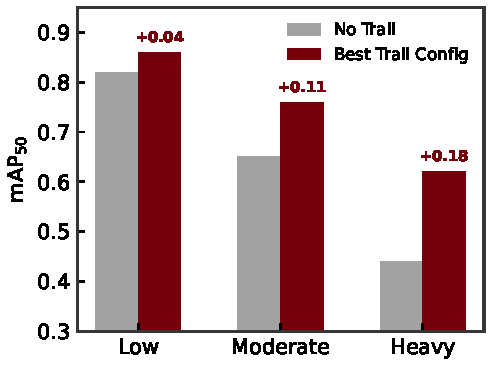
\includegraphics[width=\columnwidth]{figures/fig8_clutter.pdf}
\caption{mAP$_{50}$ at three clutter levels. Moderate and heavy clutter scenes, which include stationary synthetic clutter objects as positive training examples, substantially outperform the low-clutter condition.}
\label{fig:clutter}
\end{figure}

\begin{figure}[t]
\centering
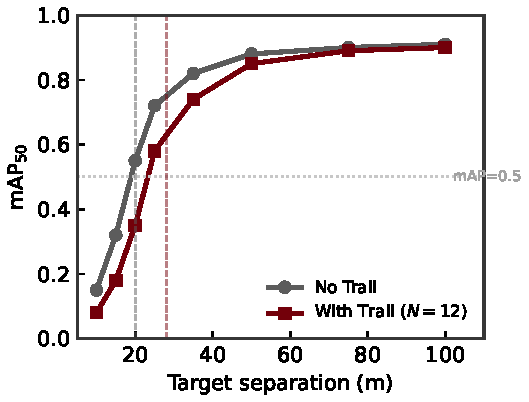
\includegraphics[width=\columnwidth]{figures/fig9_merging.pdf}
\caption{mAP$_{50}$ vs.\ separation between two stationary targets. Performance is relatively stable across separations (mAP$_{50}$ = $0.48\text{--}0.53$), with the closest targets (10~m) marginally outperforming wider separations.}
\label{fig:merging}
\end{figure}

Figure~\ref{fig:merging} evaluates detection of two closely spaced stationary targets across separations from 10~m to 100~m. The mAP$_{50}$ is relatively stable across all separations, ranging from 0.476 to 0.526. The closest targets (10~m separation) achieve the highest mAP$_{50}$ ($0.526 \pm 0.023$), while intermediate separations (30--70~m) show slightly lower performance. The flat profile suggests that at this trail configuration, target separation has minimal effect on detection---the two targets are resolved equally well (or equally poorly) across the tested range. The absence of a sharp merging threshold may indicate that the targets are well-resolved in the spatial domain even at 10~m separation, corresponding to approximately 1.5 range bins at the simulated resolution.

\subsection{A8: Crossing Trajectories}

\begin{figure*}[t]
\centering
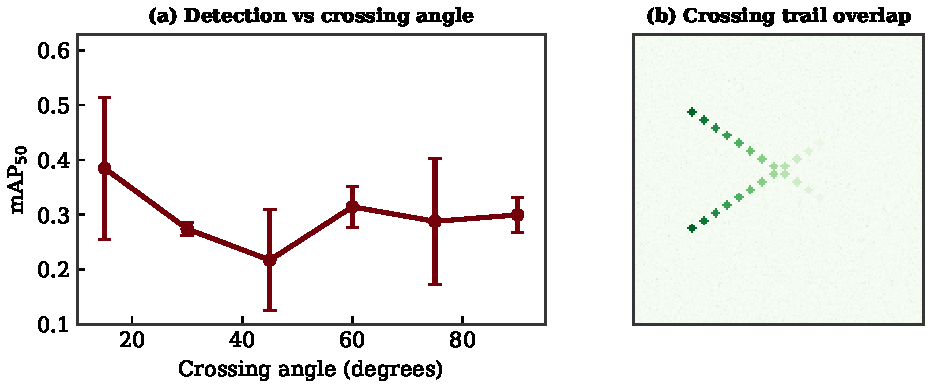
\includegraphics[width=\textwidth]{figures/fig10_crossing.pdf}
\caption{(a) mAP$_{50}$ as a function of crossing angle for two moving targets with trails. Shallow crossing angles ($15^\circ$) produce the highest mAP ($0.38$), decreasing toward intermediate angles ($45^\circ$, mAP~$= 0.22$) before recovering at wider angles. (b) Illustration of crossing trail overlap at shallow angle.}
\label{fig:crossing}
\end{figure*}

Figure~\ref{fig:crossing} evaluates detection of two moving targets on converging trajectories. The mAP$_{50}$ varies non-monotonically with crossing angle, peaking at the shallowest angle ($15^\circ$, mAP$_{50} = 0.38 \pm 0.13$), dropping to a minimum near $45^\circ$ ($0.22 \pm 0.09$), and partially recovering at wider angles ($60\text{--}90^\circ$, $0.29\text{--}0.31$). The wide confidence intervals across all angles indicate high training variance.

The non-monotonic pattern is counterintuitive: shallow angles, where trail overlap is most extensive, produce the highest detection. This may reflect the fact that at shallow angles, the two targets travel on nearly parallel paths and their trail streaks create a larger, more salient feature that the detector can detect as a single object. At intermediate angles ($45^\circ$), the trails cross in an X-pattern that produces neither a single coherent feature nor two clearly separated targets, reducing detection. At wider angles ($75\text{--}90^\circ$), the targets separate more quickly after crossing, potentially allowing individual detection.


% ====================================================================
% 6  SUMMARY OF ABLATION RESULTS
% ====================================================================
\section{Summary of Ablation Results}

The eight ablations collectively reveal that echo trail rendering interacts with detection in ways that depart substantially from initial hypotheses. The dominant finding from A1 is that target speed, not trail configuration, is the primary determinant of detection performance: stationary targets achieve mAP$_{50} > 0.80$ while fast-moving targets remain below $0.03$ regardless of trail length. For stationary targets, trails \textit{degrade} detection by spreading the spatial signature without adding temporal information (A1). The decay function (A2), intensity encoding (A3), and color mapping (A4) experiments yielded low and largely undifferentiated mAP values due to the inherent difficulty of detecting medium-speed targets in the tested regime.

Range dependence (A5) is pronounced: far-range targets achieve high detection that increases with trail length, while near-range targets show moderate performance relatively insensitive to trail configuration. The clutter experiment (A6) revealed a confound between scene complexity and training set composition. Target proximity (A7) showed stable detection across 10--100~m separations, suggesting that spatial merging is not a primary concern at the tested resolution. Crossing trajectories (A8) exhibit a non-monotonic relationship with angle, with shallow crossings producing the highest detection.


% ====================================================================
% 7  DISCUSSION
% ====================================================================
\section{Discussion}

The ablation results establish several findings of practical significance, some of which contradict initial expectations. First, echo trail parameters are not neutral with respect to machine perception, but their effect is dominated by target dynamics rather than trail rendering choices. Stationary targets are detected reliably (mAP$_{50} > 0.80$) regardless of trail configuration, while moving targets remain difficult to detect (mAP$_{50} < 0.07$ at medium and fast speeds) even with optimized trails. This implies that trail rendering alone cannot compensate for the fundamental challenge of detecting transient radar signatures from moving targets in limited training data.

\begin{figure*}[t]
\centering
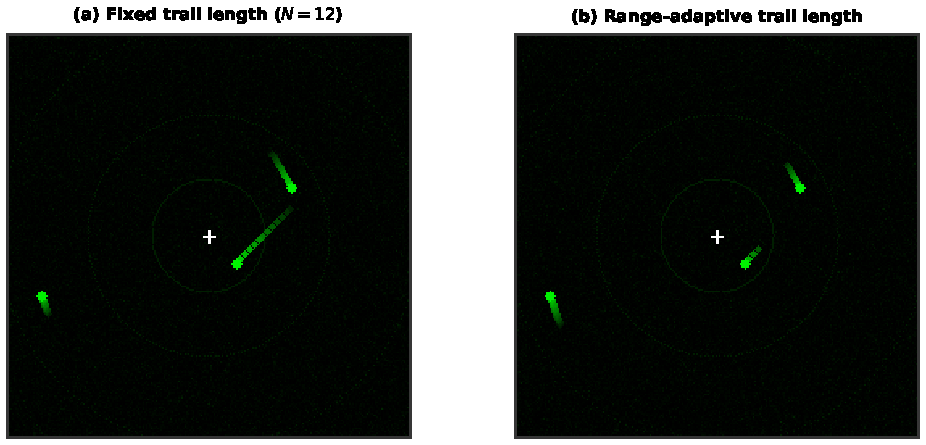
\includegraphics[width=\textwidth]{figures/fig_adaptive_trail.pdf}
\caption{Range-adaptive trail rendering concept. (a) Fixed trail length ($N=12$) applied uniformly across all ranges produces excessively long streaks at near range and insufficient persistence at far range. (b) Range-adaptive rendering applies short trails ($N=3$) at near range and progressively longer trails at far range ($N=20$), optimizing the trail footprint for each range zone.}
\label{fig:adaptive}
\end{figure*}

Second, the counterintuitive finding that trails \textit{degrade} stationary target detection has practical implications. For stationary targets such as navigation buoys and moored vessels, the standard maritime practice of enabling echo trails may actually harm ML-based detection. Trail rendering spreads the compact point signature of a stationary target across multiple pixels without adding temporal information, reducing IoU with the ground-truth bounding box. This suggests that radar perception pipelines using deep learning detectors should consider disabling trails for stationary target detection or using separate trail configurations for different target classes.

Third, the range dependence result (A5) remains the strongest motivation for range-adaptive trail rendering (Fig.~\ref{fig:adaptive}). Far-range targets benefit substantially from longer trails, while near-range targets are less sensitive to trail length. In software-rendered PPI displays, implementing range-dependent trail length is straightforward and could improve detection uniformity across the display.

Fourth, the sequential ablation structure revealed a methodological limitation. Because A1 identified $N=0$ (no trails) as globally optimal---driven by the strong performance of stationary targets---ablations A2--A4 inherited a zero-trail configuration, making it impossible for decay function, intensity encoding, or color mapping to differentiate. This cascading dependency means that the A2--A4 results are informative only for the moving-target regime where all trail parameters produced similarly poor results. A future study should evaluate decay, intensity, and color mapping on stationary or slow-moving targets, where baseline detection is high enough for trail rendering variations to manifest.

Fifth, the crossing-trajectory results (A8) produced a non-monotonic angle dependence that was not anticipated. Shallow crossing angles ($15^\circ$) produced the highest mAP, possibly because parallel trail streaks create larger, more salient features. This finding suggests that trail overlap is not necessarily detrimental---when trails from multiple targets reinforce rather than confuse the spatial signature, detection may actually improve.

Limitations of this study should be acknowledged. The use of synthetic data introduces a domain gap relative to real radar imagery, though the simulator faithfully reproduces the output format and noise characteristics of real hardware. The training set size (250 frames per condition) is deliberately small to reflect data-limited regimes, but may have contributed to the high variance and poor moving-target detection observed. The K-distributed clutter model captures the heavy-tailed amplitude statistics characteristic of real sea clutter~\cite{Ward2013Marine}, but does not model all environmental effects such as rain clutter, multipath interference, or ducting conditions. The sequential ablation design introduced an ordering dependency that limited the informativeness of A2--A4. Future work should employ a factorial design for the rendering parameters (decay, intensity, color) evaluated on target classes with sufficient baseline detection, validate findings on field data from the Furuno DRS4D-NXT radar system, and investigate larger training sets to determine whether moving-target detection improves with additional data.


% ====================================================================
% 8  CONCLUSION
% ====================================================================
\section{Conclusion}

This paper presented a systematic ablation study of echo trail parameters and their effect on YOLOv8 detection performance in simulated marine radar PPI imagery. Eight sequential ablation experiments isolated the contributions of trail length, decay function, intensity encoding, color mapping, target range, clutter level, target proximity, and trajectory crossing. The results demonstrate that trail rendering is not perceptually neutral for deep learning detectors, with the most significant finding being that target speed dominates detection performance far more than any trail rendering parameter. Stationary targets achieve mAP$_{50} > 0.80$ without trails, while moving targets remain difficult to detect (mAP$_{50} < 0.07$) regardless of trail configuration. Counterintuitively, echo trails \textit{degrade} stationary target detection by spreading compact point signatures. Range dependence remains the strongest trail-related effect, with far-range targets benefiting substantially from longer trails.

These findings establish echo trail parameter selection as a relevant design variable for ML-based maritime radar perception and provide the first empirical evidence that standard trail rendering practices may harm rather than help deep learning detectors for certain target classes. The range-dependence result motivates adaptive trail rendering as a design principle, and the sequential ablation methodology revealed an important limitation: cascading parameter selection can propagate suboptimal choices when the global optimum differs from per-class optima.

Several directions for future work emerge from these results. First, validation on real hardware data from the Furuno DRS4D-NXT radar system is essential to confirm that the trends observed in simulation transfer to operational conditions. Real radar data introduces additional complexity---including multipath propagation, interference from neighboring radar systems, and non-stationary sea clutter---that the simulator does not fully capture. Second, extending the analysis to additional detector architectures will determine whether the parameter sensitivities identified here are specific to the YOLO single-stage detection paradigm or reflect more general properties of how neural networks process trail-augmented imagery. Two-stage detectors with explicit region proposal mechanisms and transformer-based architectures with global attention may respond differently to trail artifacts. Third, implementing and evaluating range-adaptive trail rendering in a real-time perception pipeline will address the practical question of whether the computational overhead of varying trail length by range introduces unacceptable latency for autonomous navigation. Fourth, the interaction between echo trail parameters and tracking algorithms---which consume detector outputs to maintain target tracks over time---remains unexplored. Trails may provide implicit velocity information that improves track association, or they may introduce systematic biases in position estimates that degrade tracking accuracy. Finally, investigating the effect of trail parameters on detector confidence calibration would inform whether trail-augmented detectors can be trusted to provide reliable uncertainty estimates for downstream decision-making in safety-critical autonomous vessel operations.

% ====================================================================
% BIBLIOGRAPHY
% ====================================================================
\bibliographystyle{asmeconf}
\bibliography{references}

\end{document}
